\documentclass[noanswers, addpoints, 12pt]{exam}
\usepackage[utf8]{inputenc}
\usepackage[french]{babel}
\usepackage[T1]{fontenc}
\usepackage{xcolor}
\usepackage{listings}
\usepackage{graphicx}
\usepackage[most]{tcolorbox}

\newcommand\emptybox[1]{%
 \hbox{\smash{\hspace*{\dimexpr-\hoffset}%
  }\framebox(\textwidth, #1){}}}

\definecolor{codegreen}{rgb}{0,0.6,0}
\definecolor{codegray}{rgb}{0.5,0.5,0.5}
\definecolor{codepurple}{rgb}{0.58,0,0.82}
\definecolor{backcolour}{rgb}{0.95,0.95,0.92}
 
\lstdefinestyle{mystyle}{
    backgroundcolor=\color{backcolour},   
    commentstyle=\color{codegreen},
    keywordstyle=\color{magenta},
    numberstyle=\tiny\color{codegray},
    stringstyle=\color{codepurple},
    basicstyle=\footnotesize,
    breakatwhitespace=false,         
    breaklines=true,                 
    captionpos=b,                    
    keepspaces=true,                 
    numbers=left,                    
    numbersep=5pt,                  
    showspaces=false,                
    showstringspaces=false,
    showtabs=false,                  
    tabsize=2
}
\lstset{style=mystyle, language=Python}

\title{\vspace{-2cm}Examen Première NSI - Listes}

\date{}


\begin{document}
\runningfooter{}{\footnotesize Babash - NSI Tani Malandi et Johanne Bakalara \textperiodcentered{} CC BY-SA 4.0 \textperiodcentered{} page \thepage}{}
\firstpagefooter{}{\footnotesize Babash - NSI Tani Malandi et Johanne Bakalara \textperiodcentered{} CC BY-SA 4.0 \textperiodcentered{} page \thepage}{}

\maketitle

\pagestyle{headandfoot}
\thispagestyle{headandfoot}
\firstpageheader{Nom : \\  Prénom :\\ Classe :}{}{}
\vspace{-3cm}


\section*{Consignes:}
\begin{center} 
\fbox{\parbox{\linewidth}{
\begin{center}
Le devoir est à rédiger sur feuille libre.\\
La clarté de la rédaction et les explications font partie intégrante de la notation. Pour les questions demandant du code, respectez la syntaxe Python et soyez attentifs aux détails.
\end{center}


}}
\end{center}

\vsword{Note}
\hsword{Note}

\section*{Barème :}
\begin{center}
  \par\bigskip
  \gradetable[h]
\end{center}
\begin{questions}


\section{Liste : manipulation élémentaires}

\question[4] Questions de cours :
\begin{parts}
    \item Donner la commande permettant de créer une variable \textit{l} de type liste, contenant les valeurs 1, 3 et 5
    \item Soit \textit{l} une variable de type liste quelle commande permet d'afficher la longueur de \textit{l} ?
    \item Soit le code suivant :
\begin{lstlisting}[language=Python]
l = [4, 2, 9]    
\end{lstlisting}
Que vaut \textit{l[2]} ?
    \item Que vaut \textit{l[-2]} ?
    \item Que vaut \textit{4 in l} ?
    \item Que se passe-t-il lorsqu'on exécute la commande \textit{l[5]} ? Expliquez ce comportement.
    \item On exécute la commande \textit{l.append(12)}, que vaut maintenant l ?
    \item On exécute la commande \textit{l.insert(1, 3)}, que vaut maintenant l ?
\end{parts}

\section{Liste : compréhension de code}

\begin{lstlisting}[language=Python]
def multiplication(tab1, tab2):
    # On verifie que tab1 et tab2 sont de meme taille
    assert len(tab1) == len(tab2)
    res = 0
    for i in range(len(tab1)):
        res += tab1[i]*tab2[i]
    return res
\end{lstlisting}
\question[1] : Quel type de parcours est présent dans le code ci-dessus ?
\question[3] : Compléter le tableau d'avancement des variables pour un appel de la fonction multiplication([10, 100, 8, 4, 1], [2, 3, 1, 5, 2]).\\
 \begin{center}
\large
\begin{tabular}{c|c|c|c|c|c|}
\textbf{Tour} & \textbf{i} & \textbf{tab1[i]} & \textbf{tab2[i]} & \textbf{tab1[i]*tab2[i]} & \textbf{res} \\
\hline
Avant & & & & &\\
0 &  &  &  & &\\
1 &  &  &  & &\\
2 &  &  &  & &\\
3 &  &  &  & &\\
4 &  &  &  & &\\
retour : \\
\end{tabular}
\end{center}

\question[2] Quelles sont les valeurs de retours de la fonction multiplication pour les appels suivants (il n'est pas demandé de faire de tableau d'avancement) : \\
\begin{itemize}
    \item multiplication([0, 0, 0, 0, 0, 0, 0, 0, 0, 0], [10, 10, 10, 10, 10, 10, 10, 10, 10, 10])
    \item multiplication([1, 1, 1, 1, 1, 1], [1, 2, 3, 4, 5, 6])
    \item multiplication([2, 3, 4], [7, 8, 9])
    \item multiplication([1 for i in range(5)], [i for i in range(5)])
\end{itemize}

\section{Liste : Concevoir des algorithmes avec des listes}

\question[3] Complétez la fonction ci-dessous en suivant les commentaires.
Cette fonction reçoit une liste de nombres et retourne deux listes :
\begin{itemize}
    \item une contenant uniquement les nombres pairs,
    \item l'autre contenant uniquement les nombres impairs.
\end{itemize}
Exemple d’entrée/sortie :
\begin{lstlisting}[language=Python]
>>> filtre_pair_impair([1, 2, 3, 4, 5, 6])
([2, 4, 6], [1, 3, 5])
\end{lstlisting}

\begin{lstlisting}[language=Python]
def filtre_pair_impair(tab):
    # Fonction qui recoit une liste et retourne deux listes une pour les pairs une pour les impairs.
    pairs = ......... # on cree une liste vide pair
    impairs = ....... # on cree une liste vide impair
    for v in ..........: # on parcours tab par valeur
        if v%2 == 0 : # si v est pair
            ............... # on ajoute v a la liste pair
        else :
            ............... # on ajoute v a la liste impair
    return pairs, impairs
\end{lstlisting}

\newpage
\section{Problème}

On suppose le problème suivant où l'on cherche à déplacer le robot dans une grille, on dispose des fonctions suivantes :
\begin{description}
    \item[gauche(x)]: Une fonction permettant de déplacer le robot de x cases vers le gauche.
    \item[droite(x)]: Une fonction permettant de déplacer le robot de x cases vers la droite.
    \item[bas(x)]: Une fonction permettant de déplacer le robot de x cases vers le bas.
    \item[haut(x)]: Une fonction permettant de déplacer le robot de x cases vers le haut.
    \item[colonne()]: Une fonction qui renvoie la colonne dans laquelle se situe le robot (par exemple : 9).
\end{description}
Pour le code suivant, si le robot part du centre, le parcours est : H8-H9-E9-E7
\begin{lstlisting}[language=Python]
droite(1)
haut(3)
gauche(2)
\end{lstlisting}  
\begin{center}
    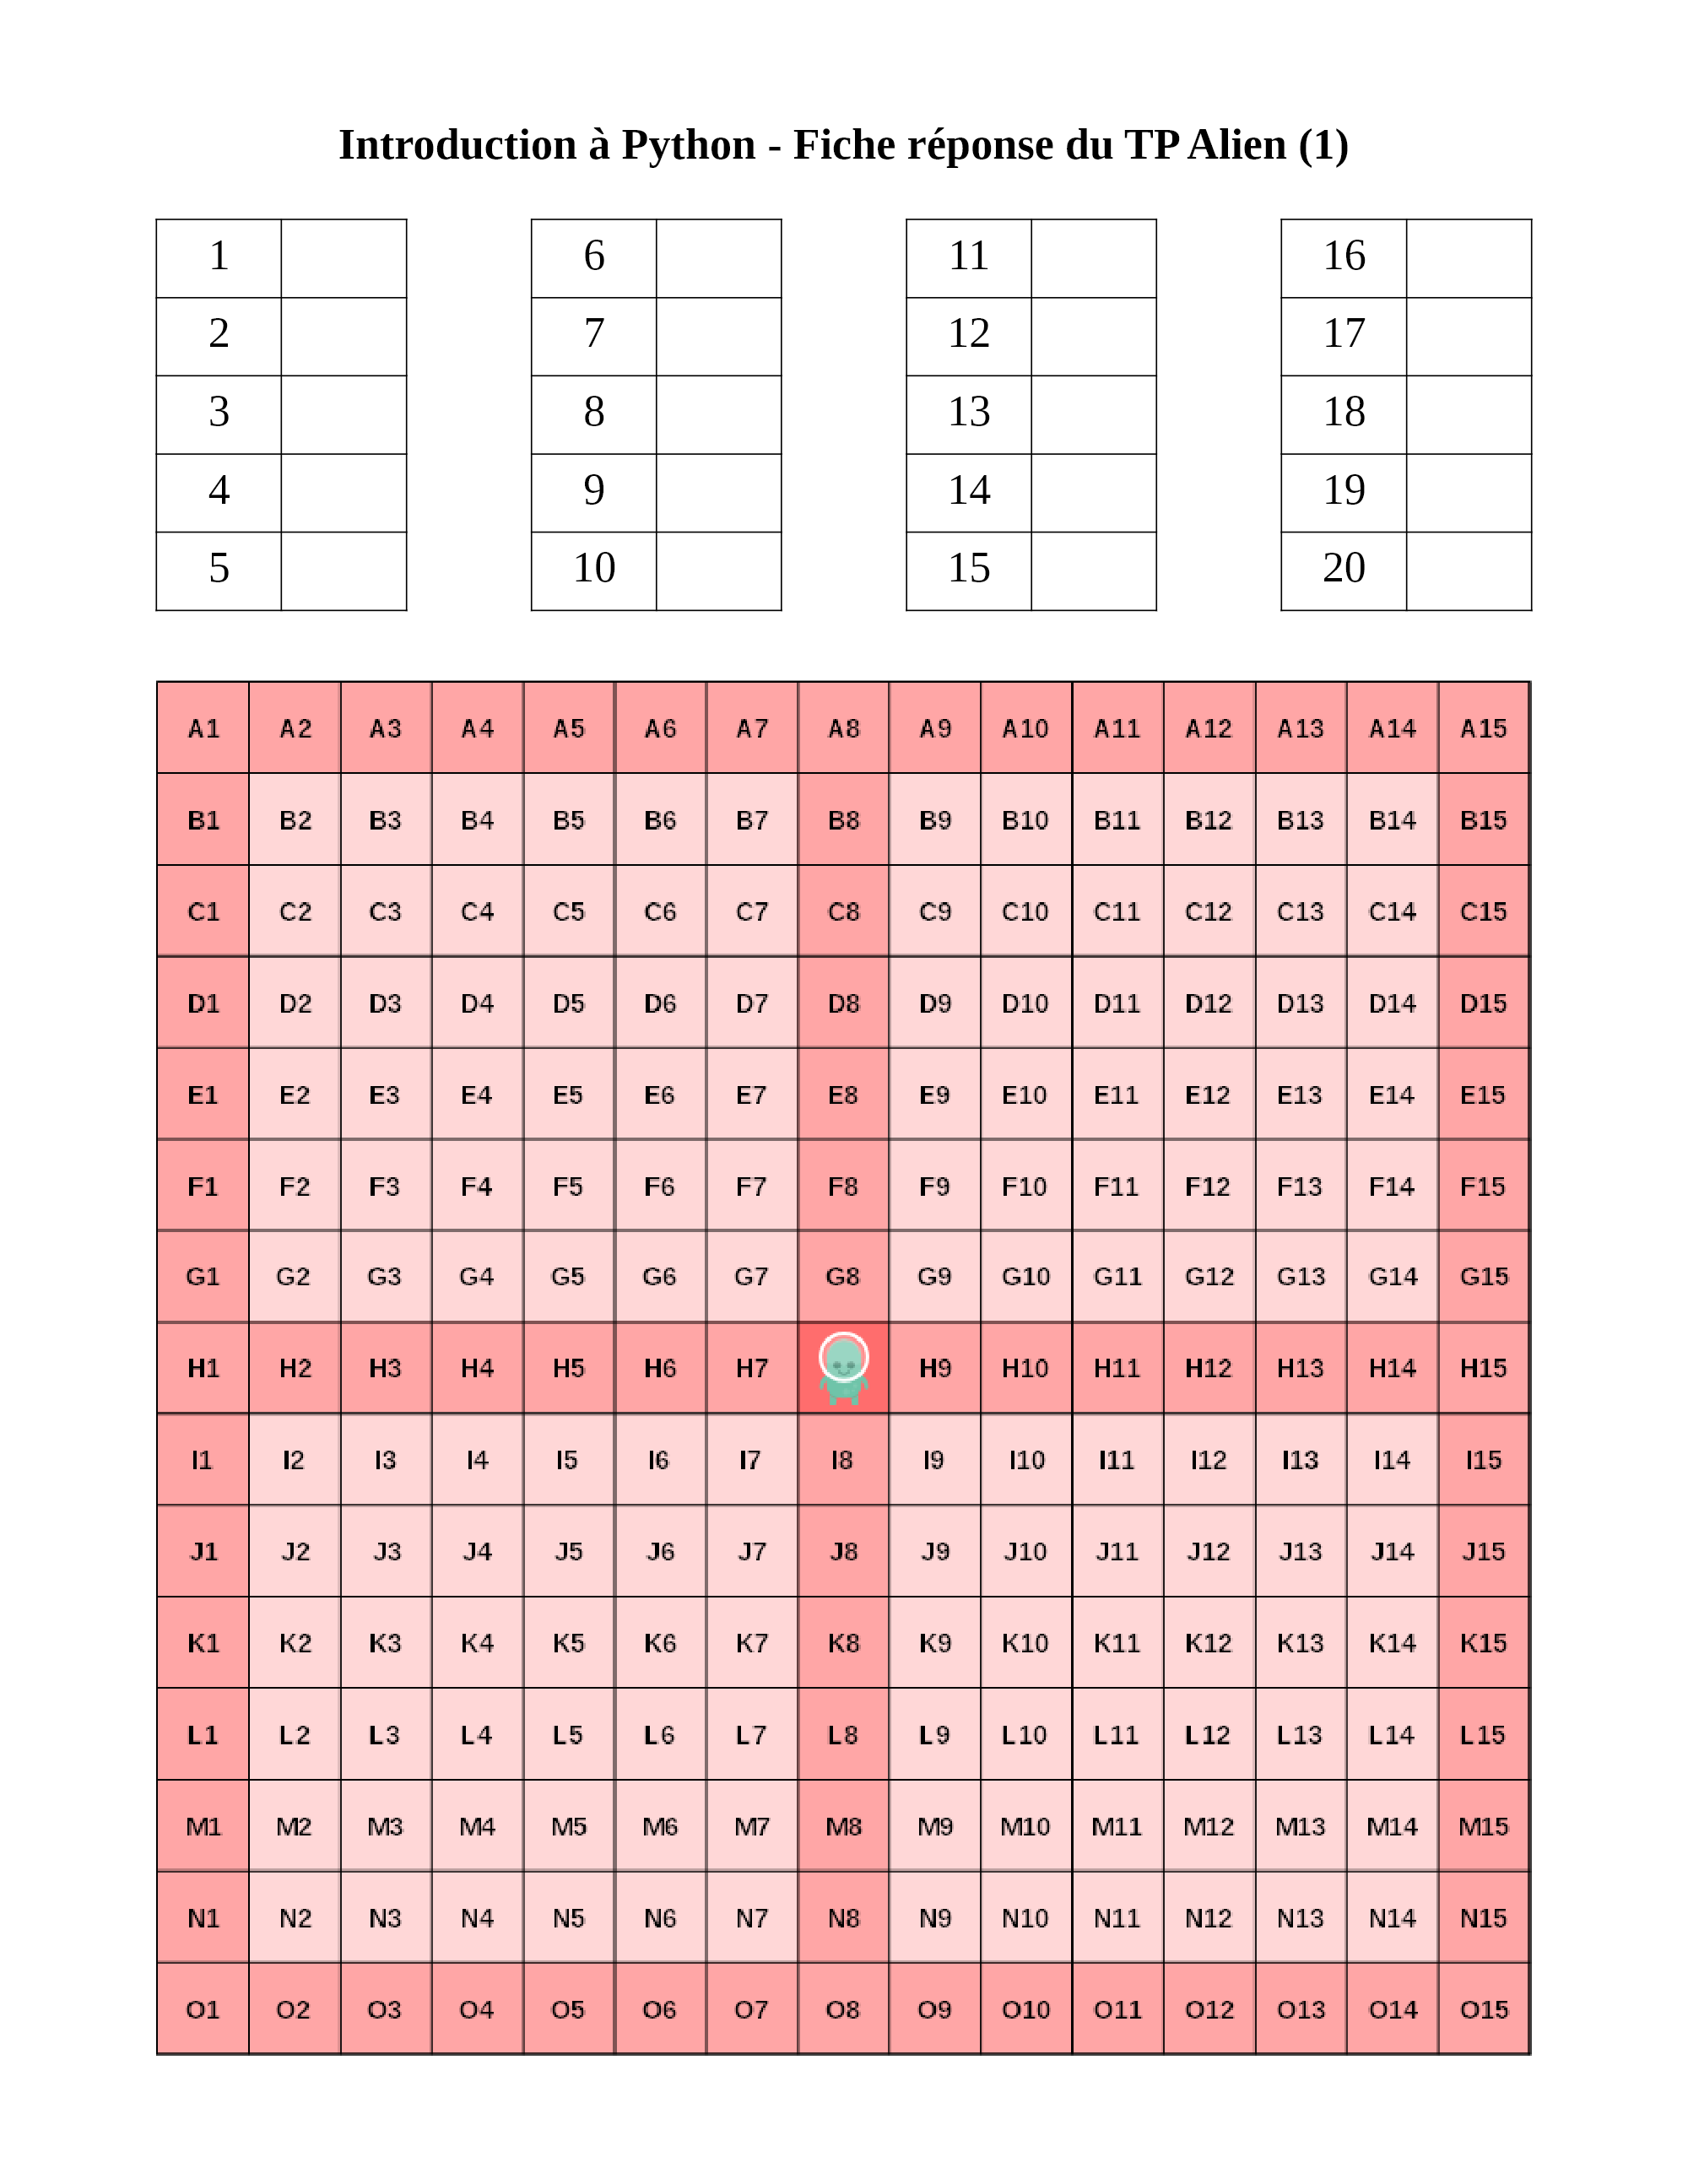
\includegraphics[width=0.85\linewidth, trim= {0 0 0 800}, clip]{BLOB/alienpdf.png}
\end{center}

Pour la suite, on considérera qu'entre chaque question le robot revient en H8 sa position initiale.
\question[1] Écrire la suite d'instructions permettant d'emmener le robot à la case G15, en partant de la case centrale.

\question[4] Donner le parcours du robot déplacement par déplacement pour chacun des codes ci-dessous.
\begin{parts}
\item \begin{lstlisting}[language=Python]
D = [3, 4, 1, 2]
a = 2
droite(D[a])
haut(D[1])
a = 1
bas(D[a])
\end{lstlisting}  

\item \begin{lstlisting}[language=Python]
D = [[3, 4],[1, 2]]
for i in range(len(D)):
    gauche(D[i][0])
    haut(D[i][1])
\end{lstlisting}  

\item \begin{lstlisting}[language=Python]
D = [3, 3, 4, 1, 2, 1]
for i in range(len(D)-1):
    if D[i] - D[i+1] > 0:
        gauche(D[i])
    elif D[i] - D[i+1] < 0:
        droite(D[i])
    else:
        haut(D[i])
\end{lstlisting}

\item \begin{lstlisting}[language=Python]
D = [3, 3, 4, 1, 2, 1]
for v in D:
    if colonne() > v:
        gauche(v)
    else:
        droite(v)
\end{lstlisting}  
\end{parts}

\begin{center}
    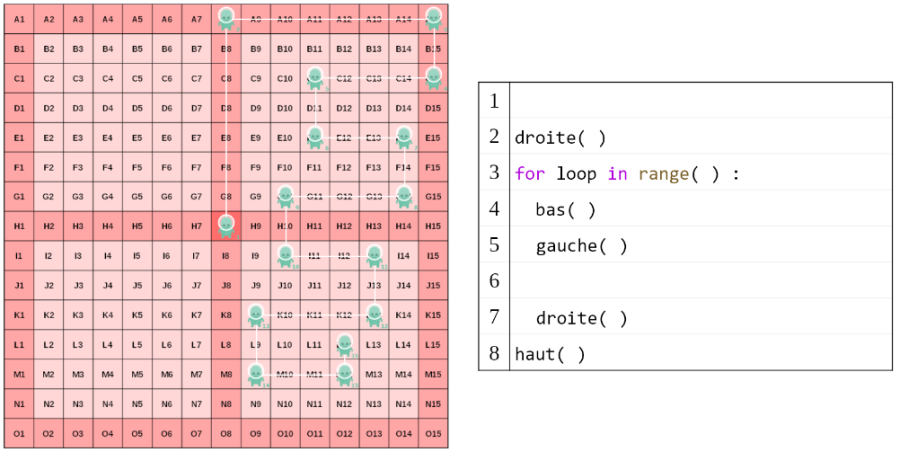
\includegraphics[width=0.5\linewidth, trim= {0 0 325 0}, clip]{BLOB/exoinverse-f268d.png}
\end{center}

\question[1] Écrire un code permettant le parcours du robot comme sur l'image ci-dessus.

\question[1] Écrire un autre code de moins de 10 lignes permettant le parcours du robot comme sur l'image ci-dessus.

\end{questions}

\end{document}

